\chapter{QoS Tools}
\section{Why QoS tools?}
In the last chapter we revised different applications with heterogeneous QoS requirements.
If all these applications coexist in the same network, it is necessary to make sure that they all see their requirements fulfilled.

One possible alternative is bandwidth overprovisioning.
If there is more than enough bandwidth, the queues are always empty and the packets suffer minimum delay and packet loss.

One of the problems of overprovisioning is that sometimes bandwidth can be very expensive.
In case of wireless communication, bandwidth is a limited natural resource.
One of the challenges of the newtwork engineers is to satisfy the QoS requirements at a reasonable cost.

Another problem of overprovisioning is the elastic demand.
Imagine that you overprovision a network to make sure that the queues are empty and the VoIP packets suffer no queueing delays.
Some users will notice that the network is blazing fast.
``Hey, I can download a HD movie in no time, I will download many of them so I can choose which one I want to watch.''
It is normal that users respond to bandwidth availability by consuming extra bandwidth.

Finally, and very similar to the previous case, there are network security threats such as worms that will consume as much bandwidth as it is available.
Sometimes a defective or misconfigured device will also consume as much bandwidth as it is available.

For all these reasons, overprovisioning cannot be the answer to everything.
An alternative to overprovisioning is to use QoS tools to manage the available bandwidth in such a way the different QoS requirements can be met by prioritizing one traffic over the others and shaping the traffic flows.

Using the road analogy, if we have an ambulances with strict delay constraints, we can make the roads wider or use prioritization and other road traffic flow management (such as traffic lamps and reversible lanes).

A QoS solution classifies the traffic into different classes accordingly to SLA requirements and treats each of these classes differently across the network.
Each of these classes is a ``class of service'' (CoS).

\subsection{Backup and maintenance}

Private users normally have Internet access with no QoS guarantees.
They pay for a 20 Mbps ADSL line, but how much they can get out of it is unknown.

Business users often choose a service with QoS guarantees, which is much more expensive than the one that has no guarantees.
Furthermore, for increased reliability, it is normal that business pay for a second line for backup purposes.
As paying for two high-speed lines would be too expensive, a more economic option is to choose a slow connection for backup.

If the main (expensive) line is out of service (either due to failure or programmed maintenance), the backup line has to support all the traffic.
At this point it is important to prioritize critical business applications at the expense of others that can be delayed to another time or another day.

As an example, if web browsing is not a critical business application but access to a remote database is, the users might not be able to browse the web until the main line has been restored.
However, this fact will not seriously impact the ability of doing business as usual.


\section{QoS at different layers}
Our interest is on the provision of end-to-end QoS.
The layer that provides end-to-end (internetworking) connectivity is the layer 3.
In the TCP/IP stack, this is the IP layer.

Nevertheless, it is also worthy to know that Ethernet, WiFi (IEEE 802.11) and MPLS also include support for QoS.
Ethernet packets include three bits in the header (Priority Code Point, PCP) to specify the class of service.
MPLS tags also have three bits to indicate the priority. 
They are called EXP bits because they were in principle reserved for experimental use.

The case of WiFi is special because it is a shared medium, in which the different nodes contend to access the channel.
There is also support for QoS in the sense that it is possible for stations with priority packets to contend more aggressively.

IP packets have a byte for QoS.
Six of the bits are there to indicate the class of service, which is called ``differentiated services code point''.
The other two bits are for ``explicit congestion notification'' (ECN).

\section{IP flow, IP class}

IP packets can be grouped in flows.
As an example when you are browsing a webpage and send multiple HTTP request packets, all those packets belong to the same flow.
The headers of the packets of the same flow have three fields in common:

\begin{itemize}
\item The layer four protocol (either TCP or UDP)
\item The source and destination IP address
\item The source and destination port.
\end{itemize}

It is important that all the packets of a flow follow the same path and are stored in the same queues, to prevent packet re-ordering.

The number of IP flows traversing a network is humongous and therefore it is not possible to apply QoS on a per-flow basis.
The alternative is to group several flows with similar QoS requirements on the same ``Class of Service''.

As an example, all web traffic flows could be mapped to the same CoS.
Also flows from other application with similar requirements (IRC, email) could be included in the same CoS.

The millions of flows traversing a router are assigned to reasonable number of traffic classes, such as four or eight.
Then, the router treats each of these classes differently in what is known as the per-hop-behaviour PHB.

Having a reduced number of classes makes the implementation and configuration of router much more easier.
It makes it even possible to use automatic tools to configure and re-configure the routers of a network.

\section{QoS tools inside a router}

To achieve QoS end-to-end, it is necessary to provide QoS in all of the intermediate hops.
As an example, if we want to provide end-to-end bounded delay, it is required to provide  bounded delay in every single hop.

To offer QoS for a traffic class, we need to define the behaviour of the routers the networks for that class of traffic.
This is known as the per-hop-behaviour (PHB).

To implement this PHB, we will use a selection of QoS tools in each router.
Normally we will need more than one tool to achieve the goal.
Some of the tools that we will cover in the course are classifiers, meters, shapers, policers, queues and markers.

For each interface of the router, and for each direction, a chain of QoS tools is used.
An example is given in Fig. \ref{fig:qos-chain} which shows a QoS tools chain for the inbound and outbound interface of a router.

\begin{figure}[h]
\centering
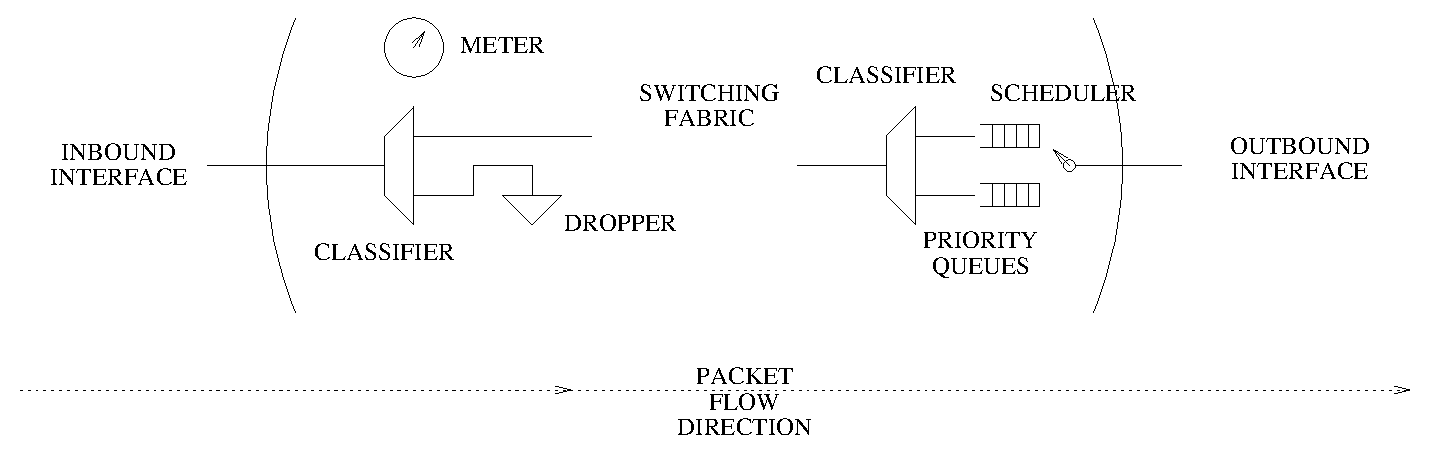
\includegraphics[width=\linewidth]{figures/qos_chain.eps}
\caption{QoS tools chain of the inbound and outbound interface of a router.}
\label{fig:qos-chain}
\end{figure}

\subsection{Classifiers}

To apply QoS, it is required to discriminate among different classes of traffic.
Therefore, the first step in any QoS tool chain is always classification.
This classification is performed by a tool that we call classifier.

These are some of the classification criteria that can be applied by a classifier:
\begin{itemize}
\item Incoming interface: Packets can be classified using the interface (either physical or virtual) that they are coming from.
As an example, we can have all the IP phones in our network in the same VLAN, and then classify the packets of this VLAN as expedited forwarding (EF).

\item Metering: We can take a classifying decision based on traffic volume.
This is typically done with token buckets (e.g. RFC 2698 \cite{rfc2698}).
Traffic conforming to a token bucket of a given rate and burst size receives a different classification than non-conforming traffic.
It is also possible to classify the traffic in three different colors (green/yellow/red) according to the CIR/PIR criteria.

\item QoS fields: We have mentioned that IP, Ethernet and MPLS packets all have a field for QoS.
The bits (the marks) in these fields can be used for classification purposes.

\item Other headers: The other headers of the packets can also be used for classification purposes.
For example, if we have a server devoted to VoIP services, we can prioritize all the packets destined to (or originated from) that server.

\item Deep packet inspection: This involves opening the packet and looking into its contents to take a decision.
It can be useful to detect signatures of virus, and identify higher layers protocols.
In the field of QoS, it is used for example to classify P2P traffic (bittorrent, kazaa).

DPI is also used for security, surveillance, espionage and censorship purposes.

\item Stateful inspection (SI): In stateful inspection we use not only information in the packet, but also information of previous packets.
As an example, it can be used to identify encrypted P2P traffic by identifying patterns such as communications with many other devices taking both the role of client and server.
\end{itemize}

DPI and SI are computationally expensive.
It would be desired to perform them only once, rather than repeating the effort in every router.
The problem is that all the classification effort is lost after the packet leaves the router, unless the QoS headers are explicitly changed.
In the next subsection we introduce the marker, which is the tool that changes QoS markings.

\subsection{Markers}

Classifying can be computationally expensive.
Additionally, some classifications can be done only at the entry point of the network.
As an example, imagine a classification based on a metering tool for the traffic of a given client.
It is feasible to use the metering tool and the classifier in the interface that the client uses to connect to the network.
However, after that traffic has been aggregated with traffic of other customers, it might not be possible isolate it with the purpose of metering.
In core routers with the larger line-speeds, only very simple (hardware based) classifications are possible.

For all these reasons, it is necessary that the routers can pass some information to each other regarding classification.
The tool for this is the marker, that changes the bits of the QoS headers of the packets.

\subsubsection{Where to classify and mark?}

Classification is done in the entry point of the network, which is also called the trust boundary.
If a network wants to identify P2P traffic to throttle it down, it will do it at the edge routers, which are the first routers that have the opportunity to inspect the packets.
Then, the QoS field of the packet headers will be marked so that other routers of the network don't have to repeat the expensive classification process.
The classification done by the other routers will be straightforward as all they have to do is to check the QoS field.

The volumes of traffic in edge routers are smaller than in core routers.
Edge routers have the necessary time to classify and mark the packets.
Edge routers also can easily differentiate traffic of different customers for metering purposes.

This initial marking may also be accompanied by policing.
A common example is to classify the traffic coming from a customer into three colors in the edge router.
Green packets are the ones conforming the CIR.
Yellow packets are the ones conforming the PIR.
And Red packets are the ones exceeding the PIR.

Red packets will be dropped (policed).
Yellow packets will be marked for drop precedence.
And green packets will be forwarded unmarked.
In case of congestion, yellow packet will also be dropped.

If the yellow packet that has been marked for drop precedence continues its trip towards its destination, it may be the victim of active queue management (AQM) tools at some later point.

\subsection{Policers}

Policers combine a meter and a dropper.
The meter is a classifier that has been explained before, and the dropper simply drops packets.
Policers play a role in enforcing CIR/PIR agreements and also in guaranteeing bounded delay for packets traversing the network, and a fair bandwidth distribution.

If an SLA defines a PIR and the customer sends traffic exceeding the PIR, the ISP will police the exceeding traffic.
A reasonable customer might police the traffic himself, to select which are the less important packets and avoid that the ISP drops packets.
Another alternative is that the customers shapes its traffic.
We will cover shapers in a later subsection.

Policers can also be used before queues.
By controlling the input rate and the size of a queue (or a set of queues) it is possible to provide delay and bandwidth guarantees to each queue.

As an example, if a queue for VoIP packets is serviced at a rate of 100 Mbps and the input is policed at a rate or 1 Mbps, with a bucket size of 100 Kbits, the  delay is bounded to $\frac{10^5 bits}{10^8 bps} = 10^{-3}s$.
Note that the delay guarantee is derived from the bucket size and not from the rate.

The rate limit is important when the voice queue is prioritized over other queues.
If the priority queue is not policed, it can starve other queues in case of misbehaviour.

Note that policers introduce packet drop but don't introduce delay.
There is a token bucket that stores tokens, but not packets.
The next subsection introduces traffic shapers that can prevent packet loss at the expense of delay.

\subsection{Shapers}

We have seen that policers drop traffic that does not conform to a given traffic profile.
An alternative of dropping is buffering.
When a shaper receives a packet and there is not enough tokens in the bucket to serve it, it will store it in a queue.
As soon as there are enough token in the bucket to serve the first packet of the queue, the shaper will allow the first packet of the queue and decrement the number of tokens in the bucket accordingly.

As the buffer size is finite, it is possible that the buffer fills up and the shaper loses packets.

Shapers are normally not appropriate for VoIP, as they introduce delay.
However they can be used to set the pace of TCP flows effectively and for this reason it is said that they are TCP friendly.

By holding packets in the buffer, the shaper increases the RTT delay.
The result is that the TCP rate is slowed down.
In the event that the buffer fills and a packet is lost, TCP halves its transmitting rate.
However, as the buffer is full, the shaper keeps transmitting at a full rate for some time and gives time to TCP to build up the congestion window and increase the transmitting rate again.

An alternative implementation of the shaper is to use a leaky bucket instead of a token bucket.
The leaky bucket simply stores packets and ``leaks'' them at a given rate.
Therefore, the leaky bucket does not allow any kind of traffic burstiness.

\subsection{Queues, droppers and schedulers}

This is a critical component of QoS.
Packets are stored in one or more FIFO queues and there is a scheduler that ``serves'' the queues by taking the first packet of a queue.
Another element of the system is the dropper, that drops packets.

There are several alternatives for the implementation of the scheduler and the dropper and we will discuss them in the next chapter.

We want to mention here that the queues do not usually contain the packets as it is much more effective to store pointers to the packets.

\subsection{The TX-ring and the interleaver}
The last element of the tools in router, just before the transmission line, is the transmission ring (TX-ring).
The normal configuration is having a queue system and the scheduler taking packets from the queues and placing them in the TX-Ring.
Differently from the queues, the TX-ring does not contain a pointer to the packet.
It contains the actual packets, ready to be transmitted.
The goal of the Tx-ring is to feed the transmission line, to make sure that it is continuously transmitting if there are packets to be serviced.
The Tx-ring is normally dimensioned in such a way that there is at least the packet that is currently under transmission and one additional packet that will follow.

The TX-ring is completely FIFO and there is no possibility to apply prioritization over the packets when they reach it.
This is not a problem in high-speed transmission lines, when transmitting a packet takes less than a millisecond.
However, in low-speed lines, the packets stored in the TX-ring can substantially delay a high priority packet.

Consider the following example.
A router transmits two kinds of traffic: VoIP and backup data.
VoIP are short (100 bytes, 800 bits) and have strict priority over backup packets, which are long (1500 bytes, 12,000 bits).
At a given point of time, the VoIP queue is empty and therefore the scheduler serves packets of the low priority queue.
The low priority queue may have a large number of packets (let's say 10) but the scheduler makes sure that there are not more than two packet in the Tx-ring.
We have a situation in which we have two long packets in the Tx-ring and a VoIP packet arrives to the high priority queue.
The VoIP packet has priority and therefore it will be the first one to be served by the scheduler.
Still, it will have to wait for the two long packets in the Tx-ring which have already been served by the scheduler.

Transmitting two 12,000 bits packets over a 1Mbps line takes around 24 ms, which is a substantial delay for VoIP packet.
To prevent this problem, an interleaver can be used in low speed link.
The idea is that long packets are divided in smaller ``chunks''.
Then, the scheduler serves chunks of a packet, instead of the whole packet.
This approach reduces the delay and jitter for high priority traffic.
